\section{Robotic Exoskeletons}
\label{sec:ExoBack}
\subsection{Introduction}

A powered exoskeleton is a wearable robotic system that offers assistive torques and increased structural support. It is an example of a Human-Machine-Interface (HMI). There has been increased interest in exoskeleton research as robotic technology has become widespread \cite{aliman2017design} \cite{chen2016recent} \cite{mertz2012next} \cite{gardner2017review}. Robotics technology has allowed smart systems to sense movement, provide feedback, and use more accurate models to produce smooth trajectories \cite{5462998}. As sensors and actuators have become more accurate and smaller, they can create lighter and more powerful exoskeletons. However, this also increases the technological difficulty in designing and building an exoskeleton. Over the years, exoskeletons have moved from simple mechanical structures to wearable robots that can sense intention and act independently. Two of the most common exoskeleton types currently being used are treadmill-based systems and overground-based systems \cite{diaz2011lower}.

Unfortunately,public spaces are not always designed to be accessible to wheelchair users. In our everyday life, we walk upstairs, reach for items on high shelves, go through narrow doorways, and talk to people at eye level \cite{welage2011wheelchair}. All of these ADLs are challenging to a person who is  confined wheelchair. Exoskeletons allow people to walk upright and live a more "normal" life. 


\subsection{Orthosis}

An orthosis is a wearable mechanism that can provide structure or power to a joint, designed to be passive or active, and have built-in sensors. A smart orthosis with actuators is classified as a robotic orthosis. Research has produced a large amount of literature on different orthotic mechanisms. Each joint in a person has different requirements and requires different technology to support and provide supplemental power. Two of the most active research areas are knee orthosis and ankle-foot orthosis. 


Several different knee orthoses designs for exoskeletons are responsible for providing power to the knee and preventing buckling. Knee orthoses are normally designed as a brake or a clutch system. Elliott \textit{et. al} presented a clutch spring knee joint for a running exoskeleton shown in \autoref{fig:runexo} \cite{elliott2014design}. This system engages and disengages the leaf spring based on the gait phase. The system holds approximately $190Nm$ with a mass of $0.710Kg$

Farris \textit{et. al} introduced a new type of brake called Wafer Disc Brakes for rehabilitation \cite{farris2009design}. The brake operates in a normally closed state that remains engaged even during a power failure, thus enabling the user's safety. The brake uses a series of stacked high-strength wafers where the stator and rotor discs are placed alternating with a relatively small distance. A motor is coupled to the center shaft. When activated, it produces a compressive force exerted via a ball screw to the discs. This setup allows the brake to hold a static torque of $73Nm$. The Austin exoskeleton project, a version control technique based on a Wrap Spring Clutch/Brake mechanism, was inherently executed to produce multiple knee joints.
 
 
 \begin{figure}[h]
    \centering
    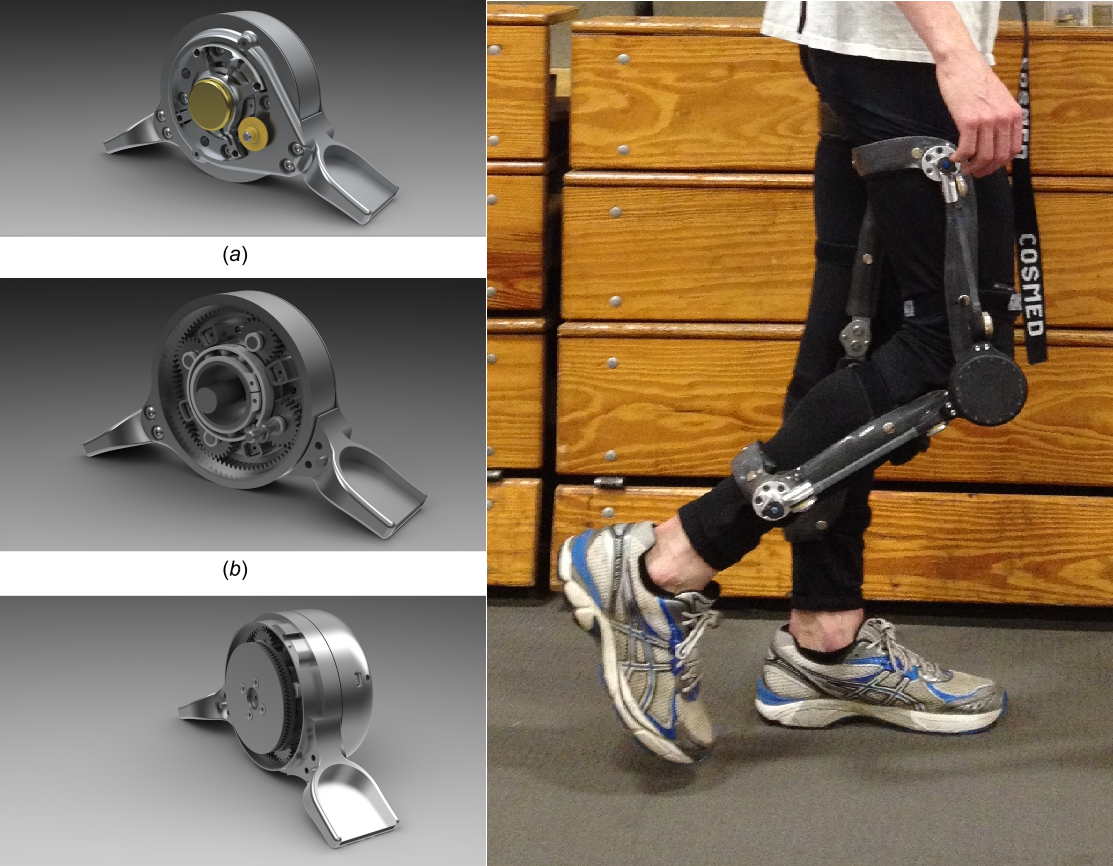
\includegraphics[scale=0.30, frame]{images/background/clutch.png}
    \caption[Clutch Spring Knee]{Clutch Spring Knee Exoskeleton for Running \cite{elliott2014design}}
    \label{fig:runexo}
\end{figure} 


Ankle-foot orthoses (AFO) designs focus on either fully active ankle actuation or on entirely restricting the motion of the foot itself. The majority of these designs are categorized as either solid ankle-foot orthoses (SAFO) or dynamic, advanced ankle-foot orthoses (DAFO) \cite{poweredAFOChina2012_6308213}. SAFOs are fully static devices designed to keep the user's foot locked at a fixed position \cite{staticAFO_6610673}. These typically consist of a single piece of plastic. DAFO devices, in contrast, consist of multiple components attached around a single adjustable hinge joint in order to avoid restricting the full range of motion of the foot \cite{poweredAFOChina2012_6308213}. DAFO designs can either be passive, non-powered devices, actively powered electrical components, or passively powered non-electrical means \cite{RussellEsposito2018}. Both actively-powered and passively-powered devices work to provide some means of controlling the angular position of the ankle throughout the gait cycle \cite{poweredAFOChina2012_6308213} \cite{actAFOFricCTRL} \cite{pneumaticAFO2009}. \autoref{fig:PAFO devices} shows some examples of different types of Powered AFO devices. An actively-powered system provides torque to aid in walking and adds mass and cost to the system.

\begin{figure}[h!]
    \centering
    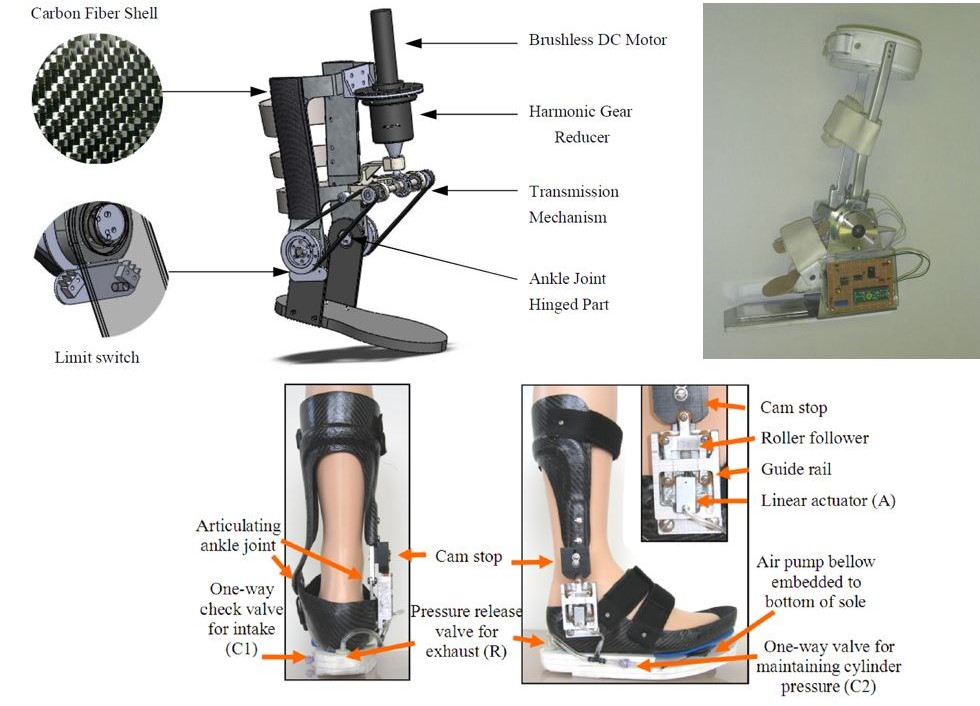
\includegraphics[scale=0.30]{images/background/PAFO_designs.JPG}
    \caption[Active v. Passive PAFO]{Various PAFO devices throughout the literature. (Top-Left) Active-PAFO (aPAFO) device that uses a motor-driven belt-chain set-up to control ankle tilt \cite{poweredAFOChina2012_6308213};  (Top-Right) aPAFO device that uses powered DC motor attached directly to the ankle-joint to control the wearer's foot \cite{actAFOFricCTRL};  (Bottom) passively-powered PAFO (PAFO) device powered by air pump attached to the sole \cite{pneumaticAFO2009}.}
    \label{fig:PAFO devices}
\end{figure} 

\subsection{Treadmill Exoskeletons}

Treadmill gait trainers, also called Body Weight Support Treadmill Training (BWSTT) or Robotically Assisted Gait Training (RAGT), typically consist of a treadmill integrated with a harness to support the person in the system and a robotic gait trainer to move the person's legs. These systems provide ample safety for the person by using a gantry and harness system to prevent falling during a trial. The control of the joint motors syncs to the treadmill's speed; this enables control of the gait speed.
 
The \textbf{Lokomat}\footnote{Hocoma AG, Industriestrasse 4, CH-8604 Volketswil, Switzerland } is a popular treadmill based exoskeleton \cite{jezernik2003robotic}. The system consists of a treadmill, a robotic orthosis, a suspension system, and two PCs. It is a 4-degree system (hips and knees). The Lokomat can be adopted for people who have had a stroke and people with SCI. An adaptive PD controller controls the joints of the exoskeleton. Several well-documented studies document the benefits of the Lokomat for rehabilitation as discussed in \autoref{sec:rehab}.
 
 
\begin{figure}[H]
    \centering
    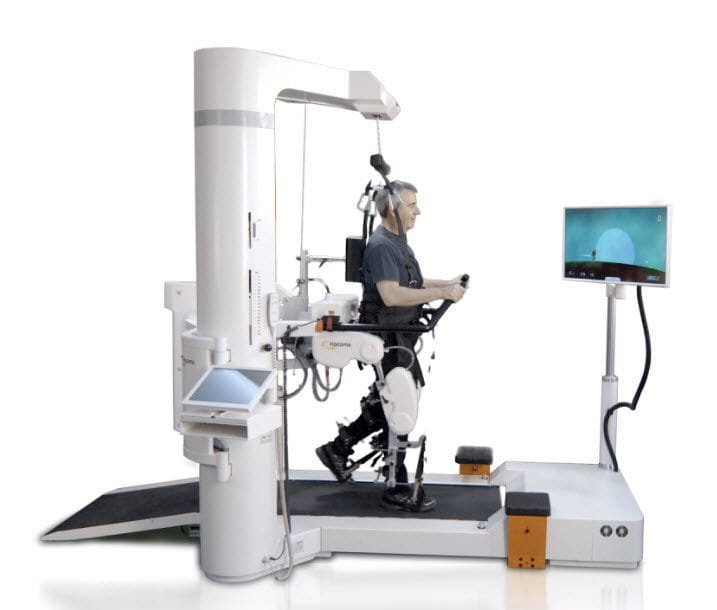
\includegraphics[scale=0.25]{images/background/loko.jpg}
    \caption[Lokomat Exoskeleton]{Lokomat Exoskeleton}
    \label{fig:loko}
\end{figure} 
 
The \textbf{Lopes} exoskeleton is another BWSTT exoskeleton. This system also uses an impedance controller to allow positional control with force interaction. This system has 8 DoF to allow hip, knee, up/down, forward/backward, and sideways freedom. Unlike many other rehabilitation exoskeletons, the actuators utilize Bowden cables for joint movement \cite{veneman2007design}. 

\begin{figure}[H]
    \centering
    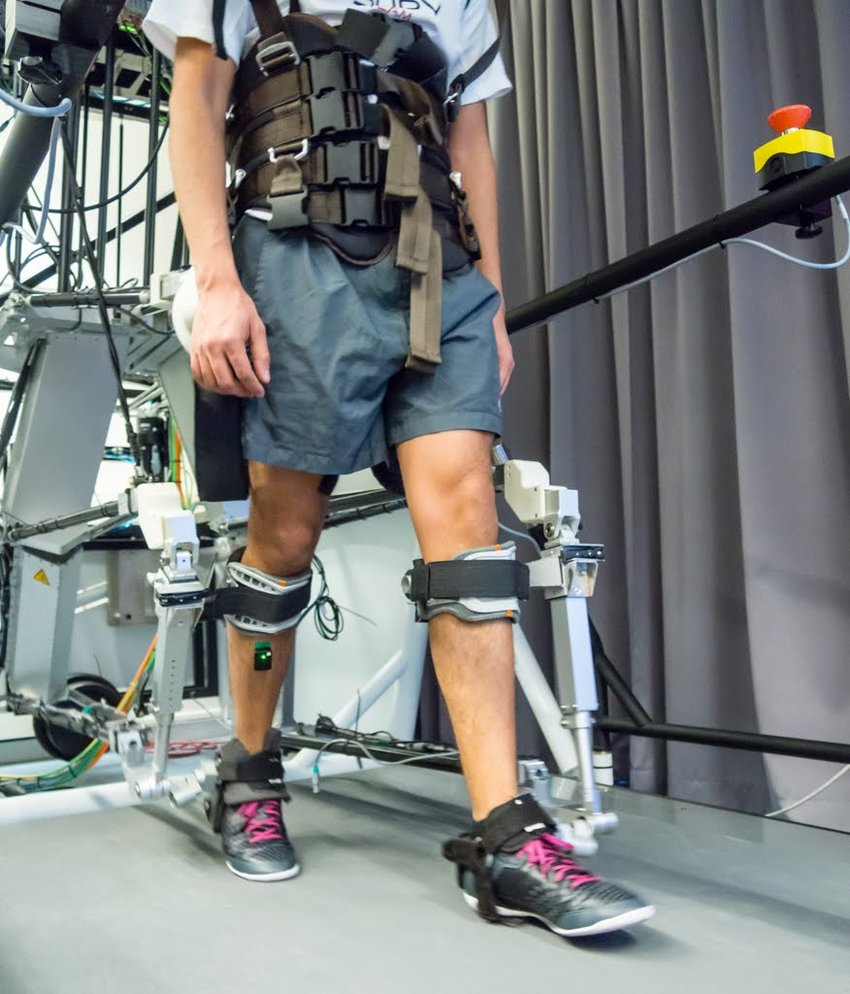
\includegraphics[scale=0.6]{images/background/A-subject-walking-with-LOPES-II-exoskeleton.jpg}
    \caption[LOPES Exoskeleton]{LOPES Exoskeleton \cite{lopes}}
    \label{fig:lopes}
\end{figure}


The disadvantage of this system is that it is not mobile. It constrains the subject to the treadmill, which does not allow for rehabilitation to involve non-level ground walking, sit-to-stand (and vice-versa), and stair climbing. Due to the support of the harness, BWSTT does not address balance recovery. It also does not have a home mode, allowing for improved daily living. Overground exoskeletons address this problem by removing the gantry systems and embedding all the actuators and controllers into the exoskeleton allowing for the freedom to move beyond a treadmill's confines.

\subsection{Overground Exoskeletons}

Several overground walking exoskeletons have been researched and developed in the past few years and have gained wide popularity. These allow for more freedom for the therapist to design protocols and represent a more realistic representation of real-world ambulation \cite{8110705} since the person is not attached to a restrictive gantry; instead, all the power and control is on-board, allowing the person to move freely in the environment. The system needs to be able to carry itself and the person. This freedom allows for movement on uneven ground and stairs. The disadvantages of these systems are that they are limited by on-board power and have to account for the system's mass. A typical design feature throughout most of the overground exoskeletons are Maxon motors\footnote{Maxon, 125 Dever Drive Taunton, MA 02780, United States}, and Harmonic gearboxes\footnote{Harmonic Drive LLC, 89 Cabot Ct # A, Hauppauge, NY 11788} \cite{bortole2015h2} \cite{aliman2017design}. The patient typically uses crutches while walking to help support the person's upper body. On average, these systems cost about \$100k \cite{rupal2017lower}.


The \textbf{BLEEX} is one of the earliest exoskeletons on the market \autoref{fig:esko} shows the current version of the BLEEX exoskeleton. The major difference between this exoskeleton and the other exoskeletons discussed in this paper is that the BLEEX design increases the load that people can carry; this was needed for military applications to help soldiers carry a substantial amount of mass. It is nearly anthropomorphic but does not quite match a person's joints. It has pure rotation joints for the knee and ball joints for the hip ankle \cite{chu2005biomimetic}\cite{zoss2006biomechanical}. The BLEEX exoskeleton focused on using clinical gait analysis for the joint design. By studying human gait motion, they were able to find the necessary design parameters for the exoskeleton, including the torques and joint ranges \cite{zoss2005mechanical}. Commercially the BLEEX became the \textbf{Ekso} exoskeleton \cite{zoss2016human}. This system cost around \$100,000 \cite{nichols_2018}. 


\begin{figure}
    \centering
    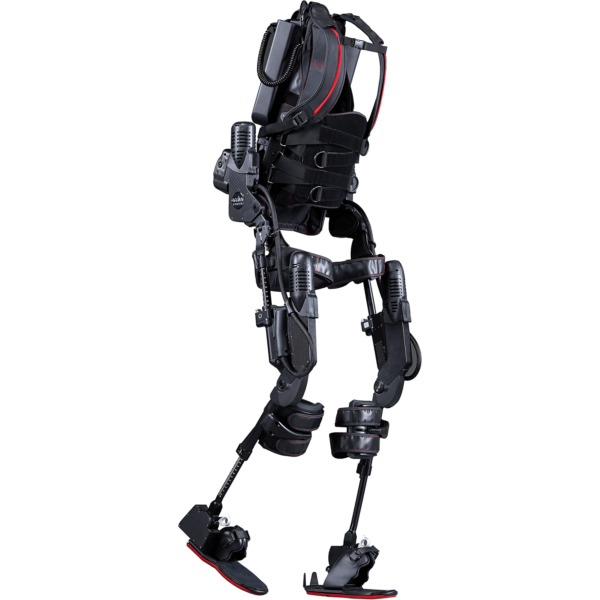
\includegraphics[scale=0.38]{images/background/ekso.png}
    \caption[Esko Exoskeleton]{Esko Exoskeleton \protect\footnote{\url{https://secureservercdn.net/72.167.25.126/045.a06.myftpupload.com/wp-content/uploads/2016/08/ekso_gt-product-image-600x600.png}}}
    \label{fig:esko}
\end{figure}


The \textbf{Rewalk}\footnote{ReWalk Robotics, Inc.
200 Donald Lynch Boulevard Marlborough, MA 01752
USA} exoskeleton is another popular rehabilitation exoskeleton on the market. \autoref{fig:rewalk} shows an image of the Rewalk. This exoskeleton has powered hips and knee joints,  the ankle joints are passive within shoe ankle support,  the control system is a closed-loop using the sensor suite to control the motors, and the body's trunk is supported with back support. The exoskeleton has several modes: sit-to-stand, stand-to-sit, up the stair, down the stair, and walking. The control of the exoskeleton is left to the user using tilt sensors in the trunk. Leaning forward tells the controller to start the walking progress  \cite{zeilig2012safety}. It is currently utilized for both inpatient therapy and at-home use. Several well-documented studies document the benefits of the Lokomat for rehabilitation as discussed in \autoref{sec:rehab}. \cite{esquenazi2012rewalk}. The home cost of the exoskeleton is approximately \$70,000 \cite{wolff2014survey}. 


\begin{figure}[H]
    \centering
    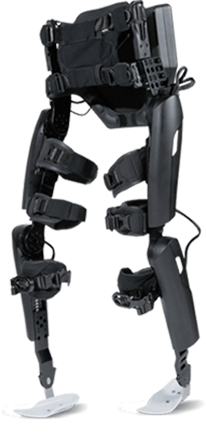
\includegraphics[scale=0.4]{images/background/rewalk-exoskelet.png}
   \caption[Rewalk Exoskeleton]{Rewalk Exoskeleton  \protect\footnote{\url{ https://rewalk.com/wp-content/uploads/2019/05/rewalk-exoskelet-6_0.png}}}
    \label{fig:rewalk}
\end{figure}


 The \textbf{Vanderbilt} exoskeleton is another popular exoskeleton for rehabilitation \cite{gasser2017design}. The market version of this system is called the Indigo exoskeleton \footnote{Parker Hannifin Corporation, Human Motion & Control 1390 E. Highland Rd. Macedonia, OH U.S.A.} shown in \autoref{fig:indigo}. This exoskeleton was first developed for post-stroke rehabilitation, where one side of the person has more function and strength than the other side. The exoskeleton provides the extra torque to help the person walk and regain strength. Recently, the Indigo exoskeleton has been used to treat people with SCI. Goldfarb \textit{et. al} has combined FES with the motorized exoskeleton for a hybrid design; this integrates the person's muscles into the system and supplements the torque with the motors \cite{ha2012enhancing}. 
 
 \begin{figure}[H]
     \centering
     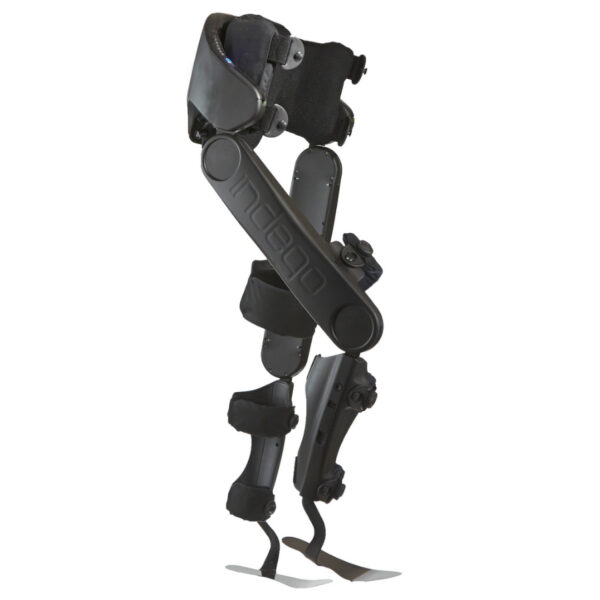
\includegraphics[scale=0.6]{images/background/Indego-via-Parker-Hannifin-Corporation-600x600.jpg}
     \caption[Indigo Exoskeleton]{Indigo Exoskeleton \protect\footnote{\url{https://secureservercdn.net/72.167.25.126/045.a06.myftpupload.com/wp-content/uploads/2016/09/Indego-via-Parker-Hannifin-Corporation-600x600.jpg}}}
     \label{fig:indigo}
 \end{figure}
 
 
 The above exoskeletons all share similar design features. They have powered hips and knees joint to provide supplementary and assistive torque, and the rigid structures provide support. The exoskeletons can be separated into several parts that can be adjusted to fit the person; this helps with the donn/doff timing and difficulty. They aid in rehabilitation by keeping the person active and bones loaded.  
 
The high price makes it difficult to purchase these exoskeletons for research and home and challenging to obtain. Justifying an exoskeleton's purchase without a proven controller is similarly difficult; testing a controller without an exoskeleton is difficult.
 
Designing and building an exoskeleton can is also expensive and time-consuming. Maxon motors can cost \$350+\footnote{\url{https://www.maxongroup.com/maxon/view/product/323772}} each  , Harmonic gearboxes can cost over a \$1000 each and require large lead times for internal reviews \footnote{\url{https://www.harmonicdrive.net/products/rotary-actuators}}. The material cost for structure can cost hundreds to thousands of dollars, including the manufacturing time. In addition, the electrical components must be custom designed to drive the motors and allow for real-time control; this, again, requires proficiency in every field of engineering, from mechanical to computer science. Additionally, a great deal of time would be spent designing, manufacturing, building, and testing the exoskeleton; this would take time and focus from designing new controllers. 
 

 

